The charged Higgs ($H^+$) decays to $c\bar{s}(\bar{c}s)$, thus the invariant mass (\mjj) of $c\bar{s}(\bar{c}s)$ pair will be the mass of the $H^+$. Reconstruction and
identification of jets coming from c-quark and s-quark is very important to reconstruct the 
mass of charged Higgs ($m_{H^+}$). We reconstruct ($m_{H^+}$) with and without kinematic fit as follows:
\begin{itemize}
    \item {\bf{$m_{H^+}$ reconstruction without kinematic fit}}: The jets are 
        reconstructed and selected as described in Sec.~\ref{s:jet_reco}. Events are
        required to have at least 4 jets. We use b-tagging as described in Sec.~\ref{s:bTag}
        to tag 2-jets as b-tagged jet. The jets are sorted in descending order of b-
        discriminator
        values and the first two jets are considered as b-jets. If an event contains exactly
        4 jets then the other 2 non-bjets are used to evaluate \mjj. However, if an
        event contains more than 4 jets, then the non-bjets are sorted in descending order of
        $\pt$ and two highest $\pt$ non-bjets are used to evaluate \mjj. The invariant 
        mass
        (\mjj) distribution after b-jet selection as described in Sec.~\ref{s:secEvtSel} is 
        shown in Figure~\ref{subfig:mjj_muBTag},~\ref{subfig:mjj_eleBTag} for data and
        background for $m_{H^+} = 100$ GeV
        and in Figure~\ref{subfig:mjj_sig_btag_mu},~\ref{subfig:mjj_sig_btag_ele} for all 
        charged Higgs
        signal samples for \mujets and electron +jets channel respectively.
    
    \item {\bf{$m_{H^+}$ reconstruction with kinematic fit}}: The kinematic 
        fit is performed on the reconstructed jets of Sec.~\ref{s:jet_reco} as
        described in Sec.~\ref{s:KinFit} in the semi-leptonic decay mode of
        \ttbar where W Boson from one of the top-quark decays leptonically 
        and W Boson from the other top-quark decays hadronically. The kinematic
        fitter also assigns jets as b-quark jets that fulfill the b-tagging
        criteria discussed before and provide the best value for the fit
        probability, these are shown in Figure~\ref{fig:feyn_diag_sig} separately
        along with other two non b-jets (coming from hadronic decay of one of 
        the W Boson). We evaluate \mjj from these two non b-jets. The 
        \mjj distribution after kinematic fit selection as described in
        Sec.~\ref{s:secEvtSel} is shown in  Figure~\ref{subfig:mjj_kfit_muKinFit}
        ,~\ref{subfig:mjj_kfit_eleKinFit} for data and background for 
        $m_{H^+} = 120 GeV$ and in Figure~\ref{subfig:mjj_sig_kfit_mu},
        ~\ref{subfig:mjj_sig_kfit_ele} for all charged Higgs signal samples for
        \mujets and \ejets channel respectively. The \mjj 
        distributions of Figure~\ref{subfig:mjj_kfit_muKinFit},
        ~\ref{subfig:mjj_kfit_eleKinFit}, and ~\ref{subfig:mjj_sig_kfit_mu},
        ~\ref{subfig:mjj_sig_kfit_ele} are used to compute the exclusion limit 
        on the $BR(t\rightarrow H^+ b)$ in Sec.~\ref{s:secLimit}.
    \end{itemize}
\begin{figure}
    \centering  
    \subfigure[\mjj with reconstructed jets \label{subfig:mjj_sig_btag_mu}]
    {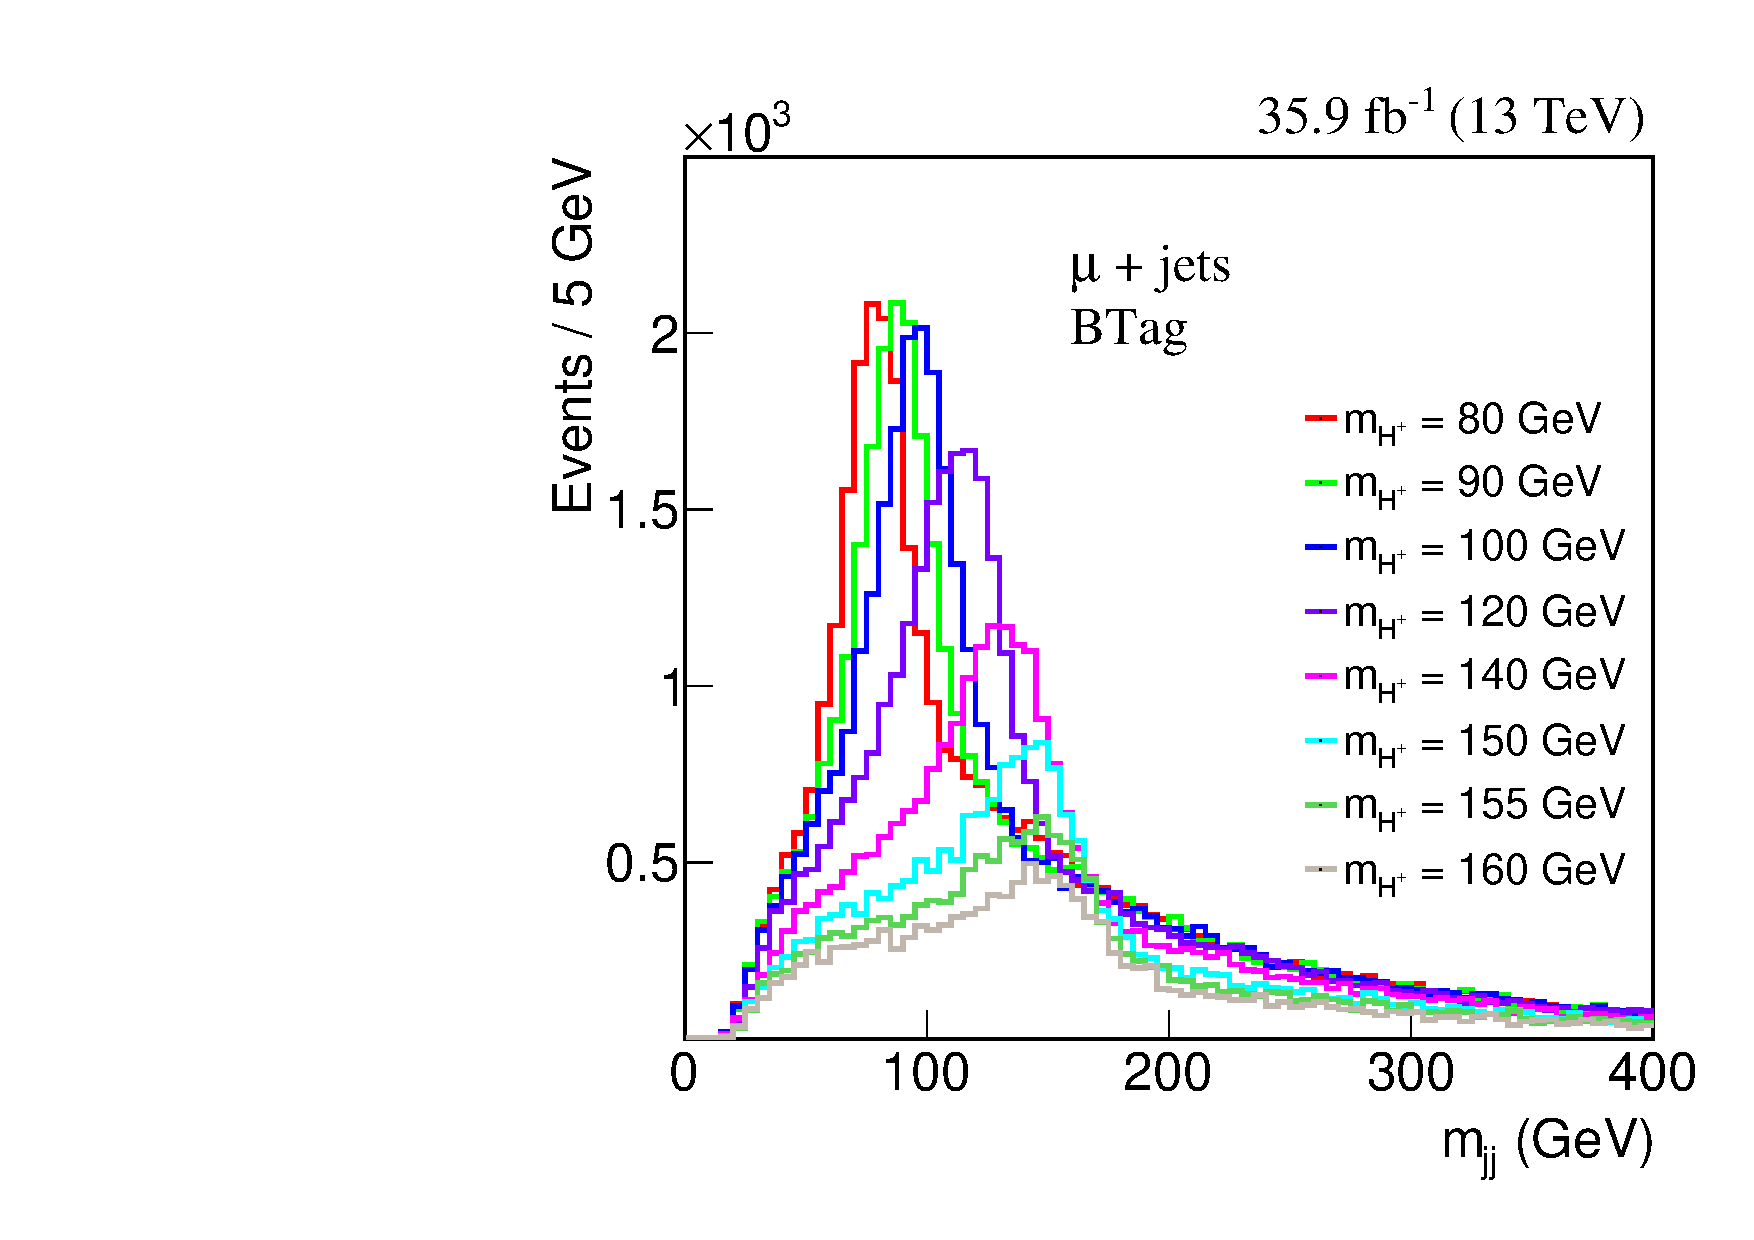
\includegraphics[width=0.45\linewidth]{Image/Muon/MjjShape_mu/sig_BTag_mjj_mu.pdf}}
    \subfigure[\mjj with reconstructed jets \label{subfig:mjj_sig_btag_ele}]
    {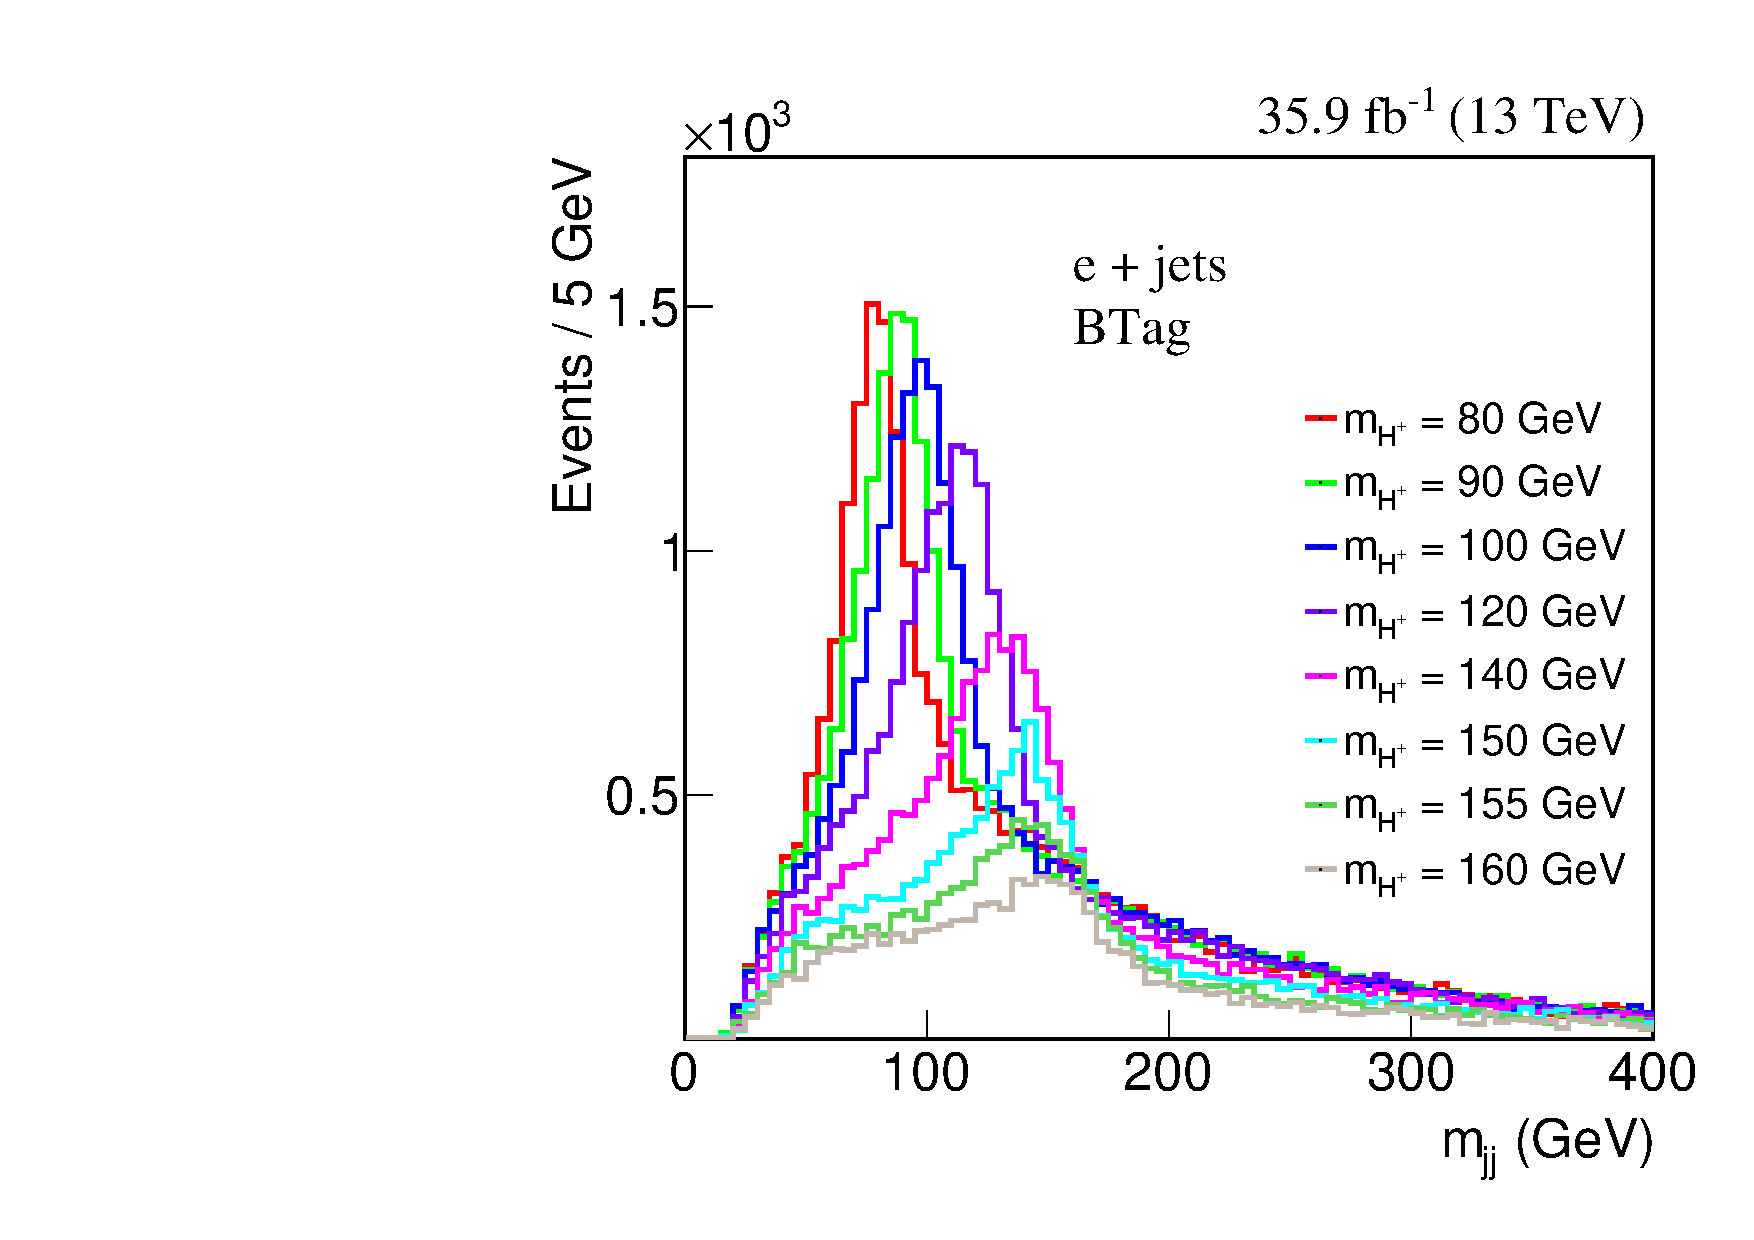
\includegraphics[width=0.45\linewidth]{Image/Electron/MjjShape_ele/sig_BTag_mjj_ele.pdf}}
    \vfil
    \subfigure[\mjj with kinematic fitted jets \label{subfig:mjj_sig_kfit_mu}]
    {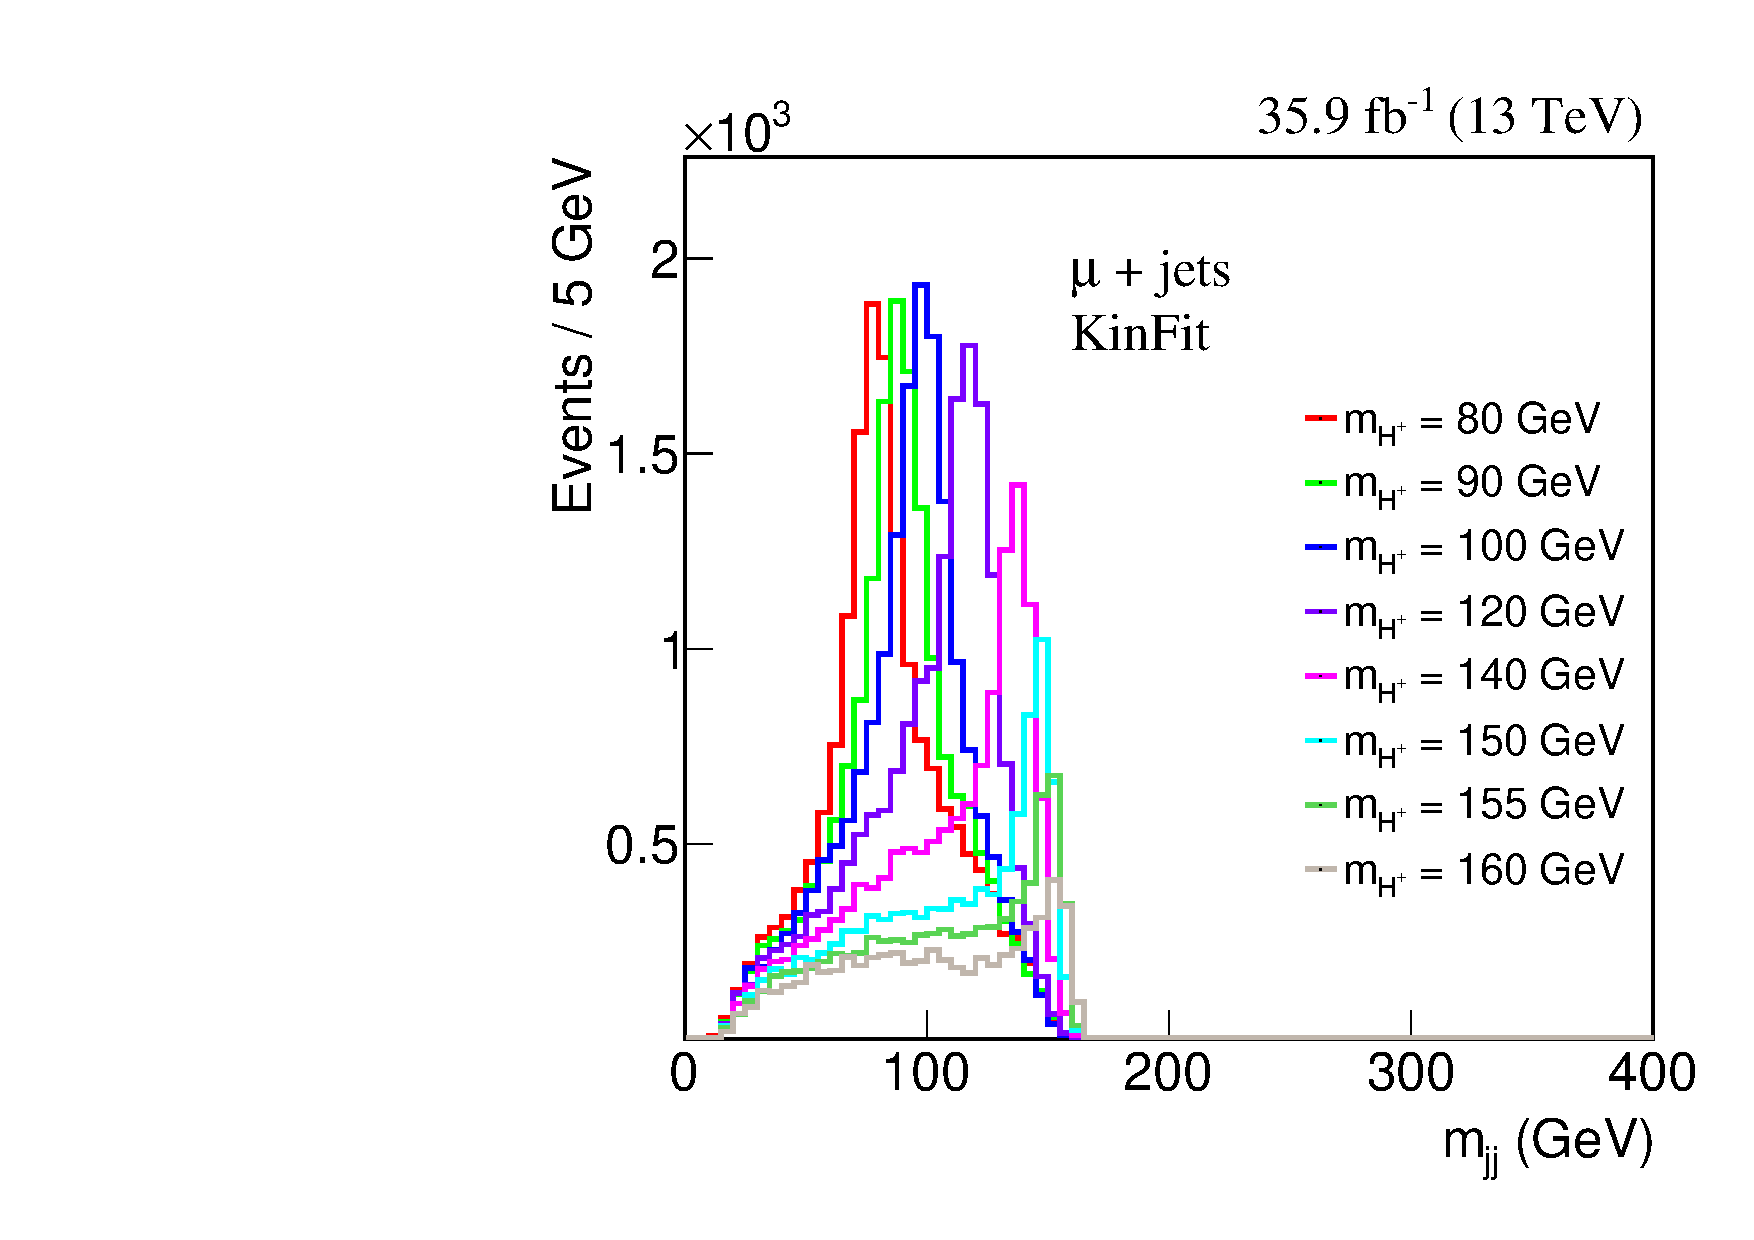
\includegraphics[width=0.45\linewidth]{Image/Muon/MjjShape_mu/sig_KinFit_mjj_kfit_mu.pdf}}
    \subfigure[\mjj with kinematic fitted jets \label{subfig:mjj_sig_kfit_ele}]
    {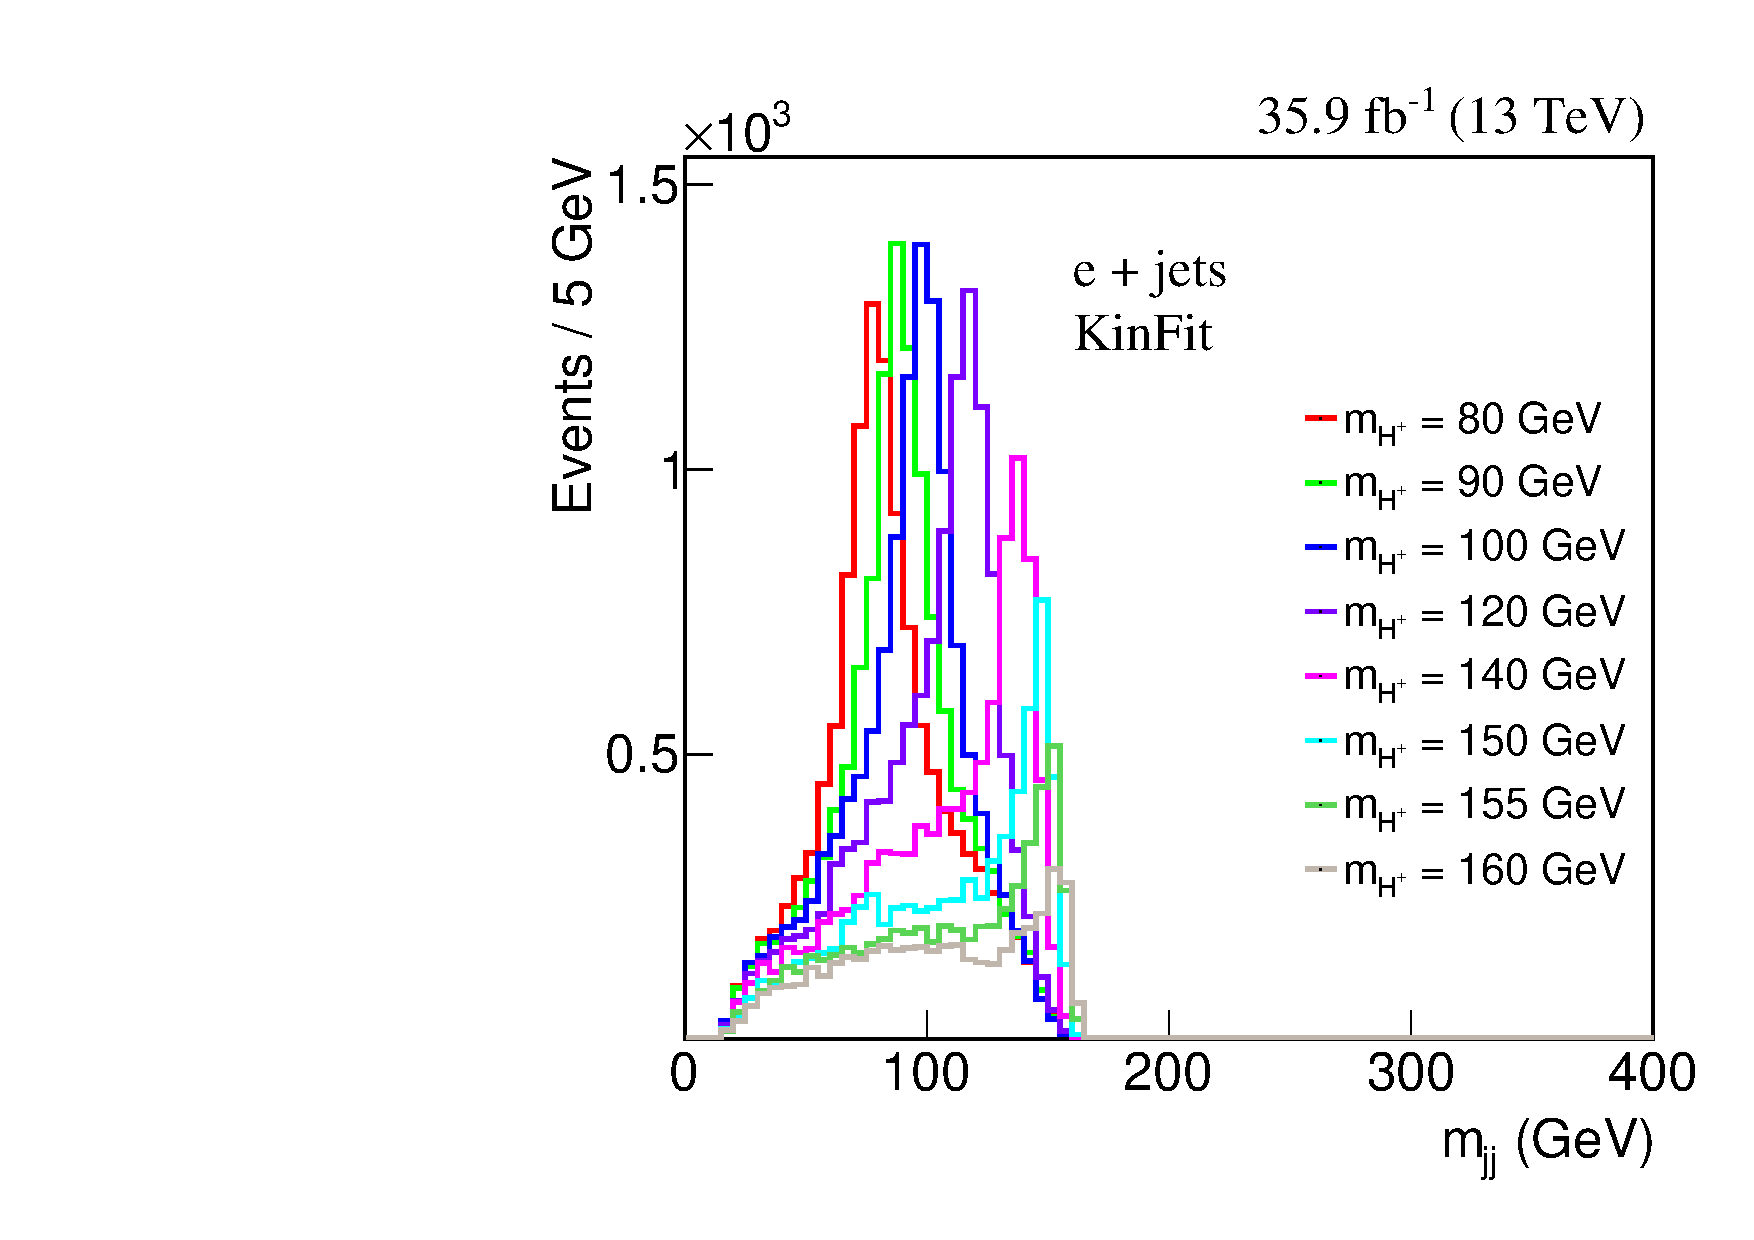
\includegraphics[width=0.45\linewidth]{Image/Electron/MjjShape_ele/sig_KinFit_mjj_kfit_ele.pdf}}
    \caption{\mjj distributions of two non-b, highest Pt-jets from charged
        Higgs signal samples ($m_{H^+}$ = 80, 90, 100, 120, 140, 150, 155, 
        160 GeV) for \mujets and \ejets channel. The \mjj
        distributions of Figure~\ref{subfig:mjj_sig_btag_mu}, 
        \ref{subfig:mjj_sig_btag_ele} are evaluated using reconstructed jets 
        after b-jet selection as described in Sec.~\ref{s:secEvtSel}. Whereas
        \mjj distributions of Figure~\ref{subfig:mjj_sig_kfit_mu}, 
        \ref{subfig:mjj_sig_kfit_ele} are evaluated using kinematic fitted 
        jets after kinematic fit selection as described in Sec.~\ref{s:secEvtSel}. 
    }
    \label{fig:mjjBTagKinFit_Sig}
\end{figure}

